%! Author = adrien koumgang tegantchouang
%! Date = 09/07/24


\chapter{Benchmarking}\label{ch:benchmarking}

For the performance tests, I have opted for an approach that consists of calculating the time required to perform the modular decomposition on a graph on two groups of graphs.
The first group are so-called simple graphs, whose number of nodes ranges from 10, 100 to 1000, from 100 to 1000 with increments of 100: $100, 200, 300, \dots, 1000$.
These graphs are said to be simple because, taking E as the set of nodes and V as the set of arcs, we have $\mid V \mid = \mid E \mid ^2 - \mid E \mid /2$.
And these are generated randomly, as shown in the graph generation python code below.
The second group are so-called complex graphs, complex because the level of connectivity (the number of arcs) of the nodes is greater than those of the first group of graphs.
For this set, we have graphs ranging from 200 nodes to 800 nodes, all with a number of arcs equal to 1000.
All these are generated and stored as dot files.

\begin{lstlisting}[language=Python, style=python, caption={Simple graph generation function}, label={lst:simple-graph-generation-function}, firstnumber=1]
    def create_two_structure(num_nodes):
        ts = TwoStructure()
        nodes = list(range(num_nodes))

        # Adding random edges with random colors
        # Arbitrary number of edges for the example
        num_edges = (num_nodes * 2) - (num_nodes / 2)
        for _ in range(int(num_edges)):
            src = random.choice(nodes)
            dst = random.choice(nodes)
            if src != dst:
                # color = random.randint(1, 2)  # Random color 1 or 2
                color = 1  # Random color 1 or 2

                # Check if the edge already exists with a different color
                existing_color = ts.color_of(src, dst)
                if existing_color == 0:  # No edge exists
                    ts.edge(src, dst, color)
                elif existing_color != color:
                    print(f"Edge {src} -> {dst} already exists with color {existing_color}, skipping...")

        return ts
\end{lstlisting}

\begin{lstlisting}[language=Python, style=python, caption={Graph complex generation function}, label={lst:graph-complex-generation-function}, firstnumber=1]
    def create_complex_two_structure(num_nodes):
        ts = TwoStructure()
        nodes = list(range(num_nodes))

        # Adding random edges with random colors
        num_edges = 1000  # Arbitrary number of edges for the example
        for _ in range(int(num_edges)):
            src = random.choice(nodes)
            dst = random.choice(nodes)
            if src != dst:
                # color = random.randint(1, 2)  # Random color 1 or 2
                color = 1  # Random color 1 or 2

                # Check if the edge already exists with a different color
                existing_color = ts.color_of(src, dst)
                if existing_color == 0:  # No edge exists
                    ts.edge(src, dst, color)
                elif existing_color != color:
                    print(f"Edge {src} -> {dst} already exists with color {existing_color}, skipping...")

        return ts
\end{lstlisting}

The TwoStructure class contains a function for creating a 2-structure from a dot file.
In this way, I ensure that I'm testing on the same graphs.


\section{Result for simple graphs}\label{sec:result-for-simple-graphs}

\begin{figure}[!h]
    \centering
    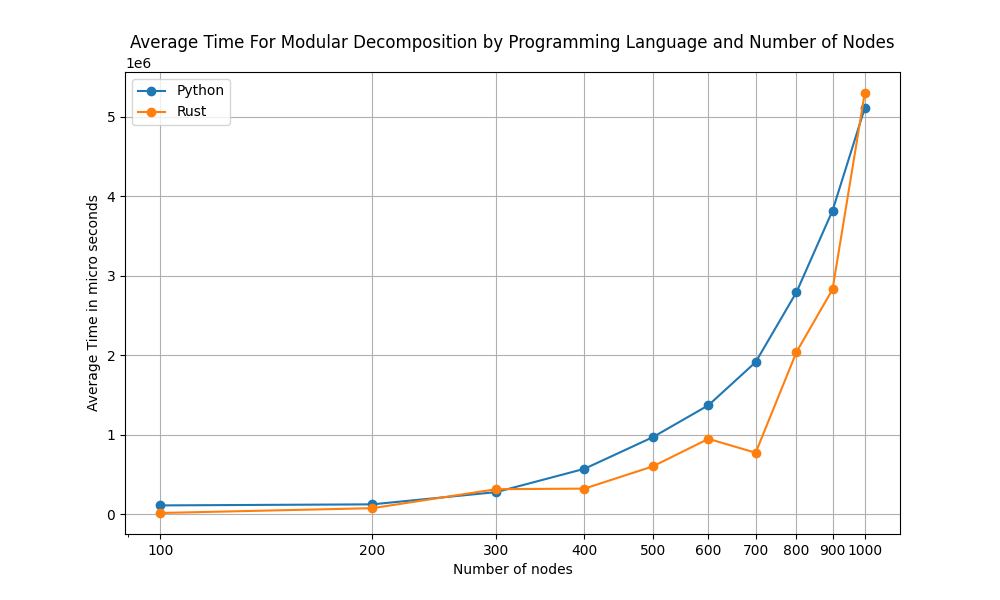
\includegraphics[width=1\textwidth]{images/stats/md_simple}
    \caption{Runtime comparison for simple graph}
    \label{fig:runtime-comparison-for-simple-graph}
\end{figure}

\section{Result for complex graphs}\label{sec:result-for-complex-graphs}

\begin{figure}[!h]
    \centering
    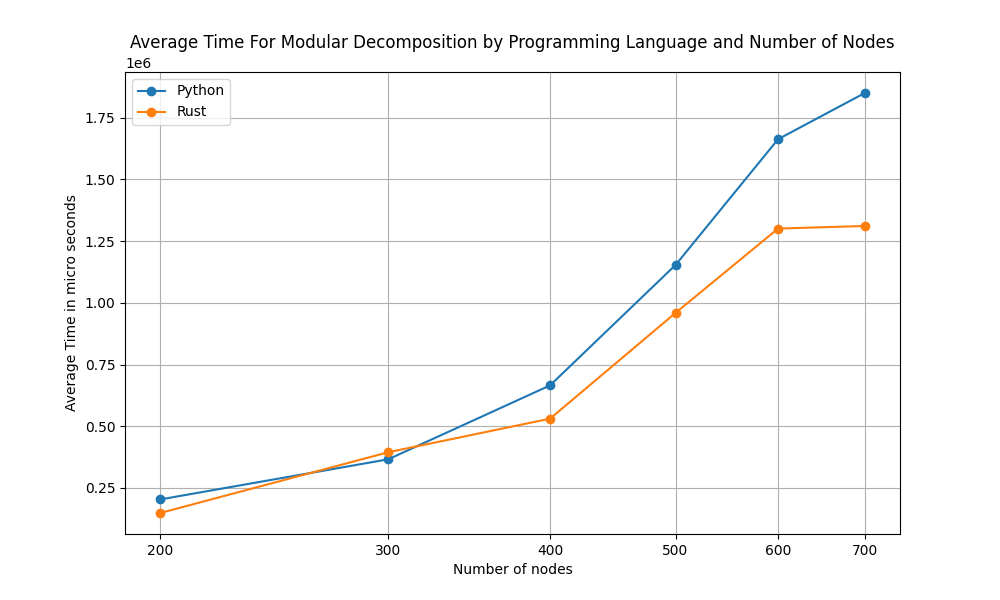
\includegraphics[width=1\textwidth]{images/stats/md_complex}
    \caption{Runtime comparison for complex graph}
    \label{fig:runtime-comparison-for-complex-graph}
\end{figure}


